%Basierend auf die Vorlage von TH Köln mit mehreren Modifizierungen

%\documentclass[12pt]{article}
\documentclass[BCOR=12mm,DIV11,titlepage,a4paper,oneside]{scrbook}
\usepackage{scrhack}
\usepackage[ngerman]{babel}
\usepackage{bibgerm}
\usepackage[utf8x]{inputenc}
\usepackage{amsmath}
\usepackage{graphicx}
\usepackage{caption}
\usepackage[colorinlistoftodos]{todonotes}
\usepackage{subcaption}
\usepackage{wrapfig}
\usepackage{setspace} 
\usepackage{svg}

% Mittels [H] können Bilder genau an einer Stelle positioniert werden
\usepackage{float}

\usepackage[breaklinks]{hyperref}

% bewirkt das HyperLinks in der PDF nicht umrandet oder farbig sind
\hypersetup{colorlinks=false}

% package for colored text
% black,white,green,red,blue,yellow,cyan,magenta
\usepackage{color}

% package for colored tables
\usepackage{colortbl}

%Paket zur Erzeugung von Anführungszeichen durch \enquote{Text}
\usepackage[ngerman]{babel}
\usepackage[babel, german=quotes]{csquotes}

%Verhindern, dass eine neue Seite für ein einzelnes Wort/Zeile verwendet wird
\clubpenalty = 10000 
\widowpenalty = 10000 

\usepackage{lipsum}
\usepackage[authoryear]{natbib}
\setcitestyle{square}

\usepackage{natbib}


\begin{document}

\begin{titlepage}
\begin{center}

\begin{figure}[!ht]
	\centering
	
\includegraphics[width=10cm]{images/tau.pdf}
\end{figure}

\vspace{0.3cm}

\begin{rmfamily}
\begin{huge}
\textbf{Optimierungen von Objekterkennungsmodellen in IR und RGB-Bildern }\\	
\end{huge}
\vspace{0.5cm}
\begin{LARGE}
Objekterkennungsmodellenoptimierungen unter verschiedenen Umweltbedingungen
\end{LARGE}
\end{rmfamily}

\vspace{0.8cm}

%Bachelorarbeit 
\begin{LARGE}
\begin{scshape}
Bachelorarbeit\\[0.8em]
\end{scshape}
\end{LARGE}

%ausgearbeitet von...
\begin{large}
ausgearbeitet von\\ 
\vspace{0.3cm}
\begin{LARGE}
Ege Çağdaş ALADAĞ\\
\end{LARGE}
\end{large}

\vspace{1.2cm}

%zur Erlangung des akademischen Grades...
\begin{large}
zur Erlangung des akademischen Grades\\
\vspace{0.1cm}
\textsc{Bachelor of Science (B.Sc.)}\\ 
\end{large}

\vspace{0.6cm}

%vorgelegt an der...
\begin{large}
vorgelegt an der\\ 
\vspace{0.2cm}
\begin{scshape}
Türkisch-Deutschen Universität\\
Fakultät für Ingenieurwissenschaften\\
\end{scshape}
\end{large}

\vspace{0.6cm}

%im Studiengang...
\begin{large}
im Studiengang\\ 
\vspace{0.1cm}
\textsc{Informatik}
\end{large}

\vspace{1.2cm}

%Autor der Bachelorarbeit und die Prüfer
\begin{tabular}{rl}
        Betreuer/in:  &  Asst. Prof. Dilek Göksel DURU\\
       					&  \small Türkisch-Deutsche Universität \\[1.0em]
\end{tabular}

\vspace{0.8cm}

%Ort, Monat der Abgabe
\begin{large}
Istanbul, im August \the\year
\end{large}

\end{center}

\newpage
\thispagestyle{empty}


\end{titlepage}


\tableofcontents
\setcounter{page}{1}
\newpage

\onehalfspacing

\chapter*{Kurzfassung}
Fügen Sie hier die Kurzfassung Ihrer Arbeit, welche bestenfalls strukturiert sein sollte, z.B. Einleitung, Hintergrund, Problemstellung, Zielsetzung, Vorgehen/Methode, Ergebnis, Fazit. 


\newpage
\chapter*{Abstract}
Hier folgt die Kurzfassung auf Englisch.

\newpage
\chapter{Einleitung}
\label{cha:Einleitung}

In the rapidly advancing field of cameras and computer vision, the development of robust object recognition models is essential for applications ranging from autonomous systems to surveillance and beyond in many different fields. As technology continues to evolve, the integration of different forms of imaging has become a key focus to enhance the adaptability and reliability of these models. Visible images are affected by environmental and illumination variations such as low lighting and sun glare; meanwhile thermal and infrared images are noisy and have low resolution. \cite[p.1]{SystematicReview23} The main advantage of thermal and infrared imagery is that they are not affected by light conditions, thus they can see objects that would otherwise be very difficult to see with visible imagery.

The increasing usage of infrared imagery \cite{InfraredCameraMarket} and AI-based object detection continuously requires better optimized and well performing detection performances, especially in difficult environmental conditions such as rainy, foggy, high and low temperatures. Improvements to these detection methods and systems can have benefits extending into fields such as autonomous vehicles, agriculture, smart cities, search and rescue operations, public safety, security and military. 








\section{Tabellen}
\label{sec:Tabellen}
Dieser Abschnitt gibt Beispiele für die Verwendung von Tabellen.

\begin{table}[ht]
    \vspace{0.5em}
	\centering
	\begin{tabular}{|l|r|}
        \hline
        Text & 12\% \\
        \hline
        Text & 34\% \\
        \hline
        Text & 56\% \\
        \hline
        Text & 78\% \\
        \hline
        Text & 90\% \\
        \hline
	\end{tabular}
	\caption[Kurztitel Tabelle]{Hier steht der lange Titel für die Tabelle}
	\label{tab:tabelle}
	\vspace{0.5em}
\end{table}

\noindent{}Dies ist lediglich ein Beispiel. Je nach beabsichtigter Aussage, können Tabellen ganz unterschiedlich aussehen. Ein weiteres Beispiel:

\begin{table}[ht]
    \vspace{0.5em}
	\centering
	\begin{tabular}{|c|l|}
		\hline
		\rowcolor[gray]{0.9}\textbf{numbers} & \textbf{text} \\
		\hline
		\hline
		1 & This text flush-left \\
		\hline
		2 & while the numbers are \\
		\hline
		3 & centred \\
		\hline
	\end{tabular}
	\caption[Alternative Tabelle]{Alternative Tabelle mit farbiger Kopfzeile}
	\label{tab:tablealternative}
	\vspace{0.5em}
\end{table}


Das Erstellen von Tabellen kann sehr aufwändig sein. Die folgenden Werkzeuge können hier sehr hilfreich sein:

\begin{itemize}
	\item Excel to \LaTeX{} Converter\\ \url{https://github.com/krlmlr/Excel2LaTeX/releases}
	\item Apple Script: Numbers to \LaTeX{} \\ \url{https://gist.github.com/pgundlach/386384}
	\item Gnumeric (hat eine Export-Funktion für \LaTeX{}): \\ \url{https://projects.gnome.org/gnumeric/}
	\item OpenOffice, Calc2LaTeX: \url{http://extensions.openoffice.org/de/project/calc2latex-macro-converting-openofficeorg-calc-spreadsheets-latex-tables}
\end{itemize}

\section{Tabellen referenzieren}
\label{sec:tabellen_ref}
In diesem Abschnitt werden die Tabellen aus dem vorigen Abschnitt im Text referenziert. Dies ist der Bezug auf die erste Tabelle \ref{tab:tabelle}, und hier der Verweis auf die zweite Tabelle \ref{tab:tablealternative}. Vergeben Sie am besten immer jeder Tabelle, Abbildung, Abschnitt, Kapitel, etc. ein individuelles label, so dass Sie dieses dann zum Referenzieren verwenden können. Im Übrigen stehen Abbildungen und Tabellen niemals für sich alleine, sondern sollten im Text diskutiert werden und somit natürlich auch referenziert. Die Verwendung des "ref{}"-Befehls sorgt dafür, dass immer auf die richtige Nummerierung verwiesen wird, selbst wenn der Text später geändert wird (z.B., wenn Tabellen hinzugefügt oder gelöscht werden). 

\section{Anführungszeichen}
\label{sec:Anfuehrungszeichen}

Es gibt verschiedene Optionen, Anführungszeichen zu generieren. Da das entsprechende Paket eingebunden wurde, können Sie folgende Optionen verwenden:

\begin{itemize}
	\item \enquote{Befehl des Pakets: csquotes}
	\item Alternativ: ``example''
	\item Oder "Beispiel". 
\end{itemize}

Wie Ihnen vielleicht aufgefallen ist, sehen die Alternative etwas anders aus. Für die Verwendung von Anführungszeichen gibt es Konventionen, siehe \url{https://de.wikibooks.org/wiki/LaTeX-W%C3%B6rterbuch:_Anf%C3%BChrungszeichen}






\newpage
%!TEX root = ../VorlageBA.tex
\chapter{Grundlagen}

\section{Digital Imagery}
Digital imagery refers to visual content in digital form, that can be recognized and displayed by computers. For the purposes of this paper, we need to make a distinction between the following image types.

\begin{itemize}
	\item{Visible Spectrum(RGB) Imagery}
	\item{Thermal(Infrared) Imagery}
\end{itemize}

\subsection{Visible Spectrum(RGB) Imagery}

\cite{nasa_visiblelight} defines the visible light spectrum as the part of the electromagnetic spectrum visible to the human eye, ranging from approximately 380 to 700 nanometers in wavelength. This range encompasses all the colors perceivable by the human eye, from violet to red.

\subsection{Thermal(Infrared, IR) Imagery}
\cite{spi_thermal} defines thermal imaging, or thermography as the detection and measuring of radiation in the infrared spectrum being emitted from an object with the use of thermographic cameras. This type of imagery can collect temperature data from its field of view and display it using a variety of color palettes. Each pixel in a thermal image represents a temperature data point, and these data points are assigned a unique color or shade based on their value, meaning that as the thermal sensor detects changes in heat energy, it will express this change by adjusting the color or shade of a pixel. \citep{flir_colorpalette}

\begin{figure}[!ht]
	\centering
		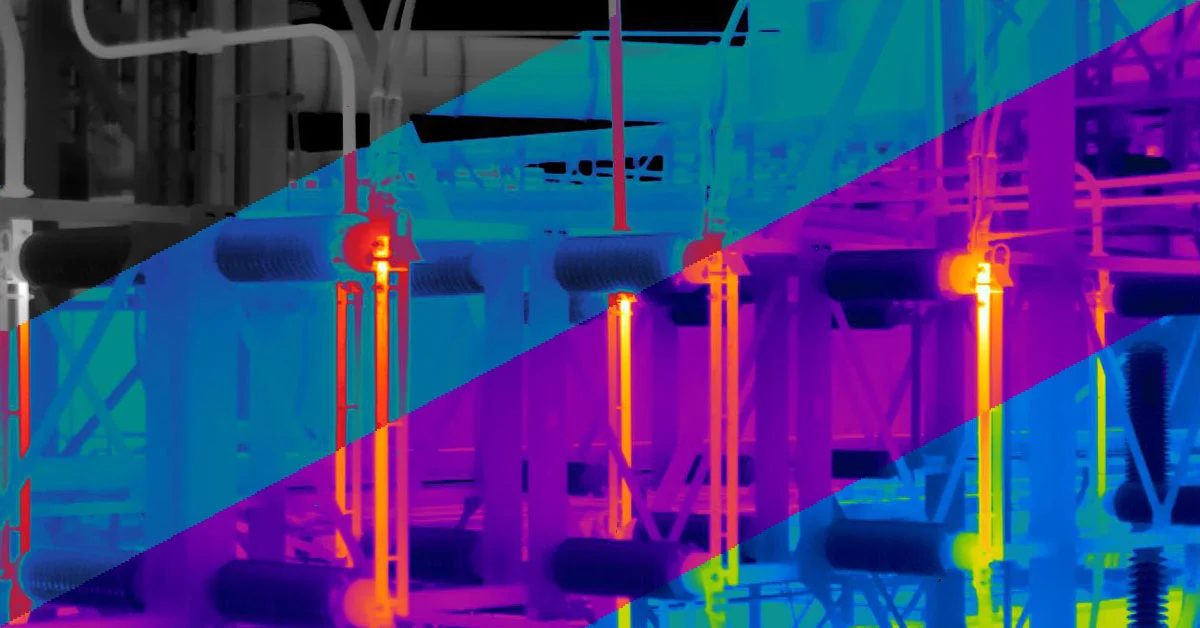
\includegraphics[width=0.75\textwidth]{images/color-palette-1200x628-fixed.png}
	\caption{Thermal Color Palettes \citep{flir_colorpalette}}
	\label{fig:color-palette}
\end{figure}

\section{Machine Learning}
\begin{quotation}
	\emph{``The studies reported here have been concerned with the
			programming of a digital computer to behave in a way
			which, if done by human beings or animals, would be
			described as involving the process of learning.''}
	\citep{samuel_machinelearning}
\end{quotation} 

Machine Learning is recognized to be a term originally coined by Arthur L. Samuel in \cite{samuel_machinelearning}. It refers to the behavior of a computer to learn by trial and error, thus improving it's performance on certain tasks over time.

For a task to be fit for a machine learning application, a definite goal must exist, and at least one criterion or intermediate goal must exist which has a bearing on the achievement of the final goal and for which the sign should be known. \citep{samuel_machinelearning} Today, machine learning systems are used to identify objects in images, transcribe speech into text, match news items, posts or products with users’ interests, and select relevant results of search. \citep{deeplearning}



\subsection{Deep Learning}
%TODO deep learning

	%TODO ML/DL optimizations

%TODO object detection

%TODO Object detection optimizations, feature selection, common algorithms and models etc.


%TODO örnek tezleri incele benzer grundlagen çıkar



\newpage
%!TEX root = ../VorlageBA.tex
\chapter{Stand Der Technik}




\newpage
%Erzeugt ein Abbildungsverzeichnis
	\listoffigures
	%Fügt die Zeile "`Abbildungsverzeichnis"' als Chapter ins Inhaltsverzeichnis ein
	\addcontentsline{toc}{chapter}{Abbildungsverzeichnis}
\newpage
	
	%Erzeugt ein Tabellenverzeichnis
	\listoftables
	%Fügt die Zeile "`Tabellenverzeichnis"' als Chapter ins Inhaltsverzeichnis ein
	\addcontentsline{toc}{chapter}{Tabellenverzeichnis}
\newpage

% To change the title from References to Bibliography:
\renewcommand\refname{Literaturverzeichnis}

%Paket für ein deutsches Literaturverzeichnis

\bibliographystyle{abbrvnat}
\bibliography{literatur} % refers to literatur.bib

	%Fügt die Zeile "`Literaturverzeichnis"' als Chapter ins Inhaltsverzeichnis ein
	\addcontentsline{toc}{chapter}{Literaturverzeichnis}
\newpage

%!TEX root = ../Masterthesis_Fischer.tex
\chapter*{Eidesstattliche Erklärung}
%\addcontentsline{toc}{chapter}{Eidesstattliche Erklärung}

Ich versichere, die von mir vorgelegte Arbeit selbständig verfasst zu haben.\\ \\
Alle Stellen, die wörtlich oder sinngemäß aus veröffentlichten oder nicht veröffentlichten Arbeiten anderer entnommen sind, habe ich als entnommen kenntlich gemacht. Sämtliche Quellen und Hilfsmittel, die ich für die Arbeit benutzt habe, sind angegeben.\\ \\
Die Arbeit hat mit gleichem Inhalt bzw. in wesentlichen Teilen noch keiner anderen Prüfungsbehörde vorgelegen.
\vspace{1.5cm}
\\
Istanbul, \today
\vspace{3cm}
\\
Max Mustermann


% chapter eidesstattliche_erklärung (end)

\end{document}
